\documentclass[12pt, oneside]{article}

\usepackage[letterpaper, scale=0.89, centering]{geometry}
\usepackage{fancyhdr}
\setlength{\parindent}{0em}
\setlength{\parskip}{1em}

\usepackage{tikz}
\usetikzlibrary{automata,positioning,arrows}

\pagestyle{fancy}
\fancyhf{}
\renewcommand{\headrulewidth}{0pt}
\rfoot{\href{https://creativecommons.org/licenses/by-nc-sa/2.0/}{CC BY-NC-SA 2.0} Version \today~(\thepage)}

\usepackage{amssymb,amsmath,pifont,amsfonts,comment,enumerate,enumitem}
\usepackage{currfile,xstring,hyperref,tabularx,graphicx,wasysym}
\usepackage[labelformat=empty]{caption}
\usepackage{xcolor}
\usepackage{multicol,multirow,array,listings,tabularx,lastpage,textcomp,booktabs}

\lstnewenvironment{algorithm}[1][] {   
    \lstset{ mathescape=true,
        frame=tB,
        numbers=left, 
        numberstyle=\tiny,
        basicstyle=\rmfamily\scriptsize, 
        keywordstyle=\color{black}\bfseries,
        keywords={,procedure, div, for, to, input, output, return, datatype, function, in, if, else, foreach, while, begin, end, }
        numbers=left,
        xleftmargin=.04\textwidth,
        #1
    }
}
{}

\newcommand\abs[1]{\lvert~#1~\rvert}
\newcommand{\st}{\mid}

\newcommand{\cmark}{\ding{51}}
\newcommand{\xmark}{\ding{55}}
 
\begin{document}
\begin{flushright}
    \StrBefore{\currfilename}{.}
\end{flushright} \section*{Day12}



{\bf Definition} A {\bf pushdown automaton} (PDA) is  specified by a  $6$-tuple $(Q, \Sigma, \Gamma, \delta, q_0, F)$
where $Q$ is the finite set of states, $\Sigma$ is the input alphabet,  $\Gamma$ is the stack alphabet,
\[
    \delta: Q \times \Sigma_\varepsilon  \times  \Gamma_\varepsilon \to \mathcal{P}( Q \times \Gamma_\varepsilon)
\]
is the transition function,  $q_0 \in Q$ is the start state, $F \subseteq  Q$ is the set of accept states.










For the PDA state diagrams below, $\Sigma = \{0,1\}$.

\vspace{-15pt}

\begin{center}
\begin{tabular}{c c}
Mathematical description of language & State diagram of PDA recognizing language\\
\hline
& $\Gamma = \{ \$, \#\}$ \hspace{2.3in} \\
& \\
& 
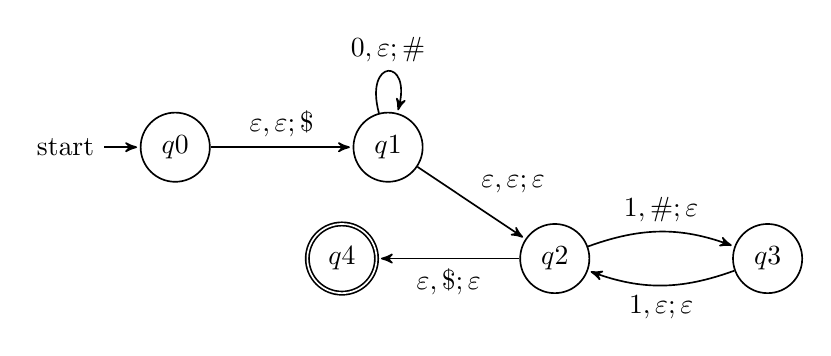
\begin{tikzpicture}[->,>=stealth',shorten >=1pt, auto, node distance=2cm, semithick]
    \tikzstyle{every state}=[text=black, fill=none]
    
    \node[initial,state] (q0)          {$q0$};
    \node[state]         (q1) [right of=q0, xshift=20pt] {$q1$};
    \node[state]         (q2) [below right of=q1, xshift=20pt] {$q2$};
    \node[state]         (q3) [right of=q2, xshift=20pt] {$q3$};
    \node[state,accepting]         (q4) [left of=q2, xshift=-20pt] {$q4$};
    
    \path (q0) edge [bend left=0] node {$\varepsilon, \varepsilon; \$$} (q1)
        (q1) edge  [loop above] node {$0, \varepsilon; \#$} (q1)
        (q1) edge [bend left=0] node {$\varepsilon, \varepsilon; \varepsilon$} (q2)
        (q2) edge  [bend left=20] node [midway, above] {$1, \#; \varepsilon$} (q3)
        (q3) edge  [bend left=20] node [midway, below] {$1, \varepsilon; \varepsilon$} (q2)
        (q2) edge  [bend left=0] node {$\varepsilon, \$; \varepsilon$} (q4)
    ;
\end{tikzpicture}
\\
& \\
& \\
\hline
& $\Gamma = \{ \sun, 1\}$ \hspace{2.3in} \\
& \\
& 
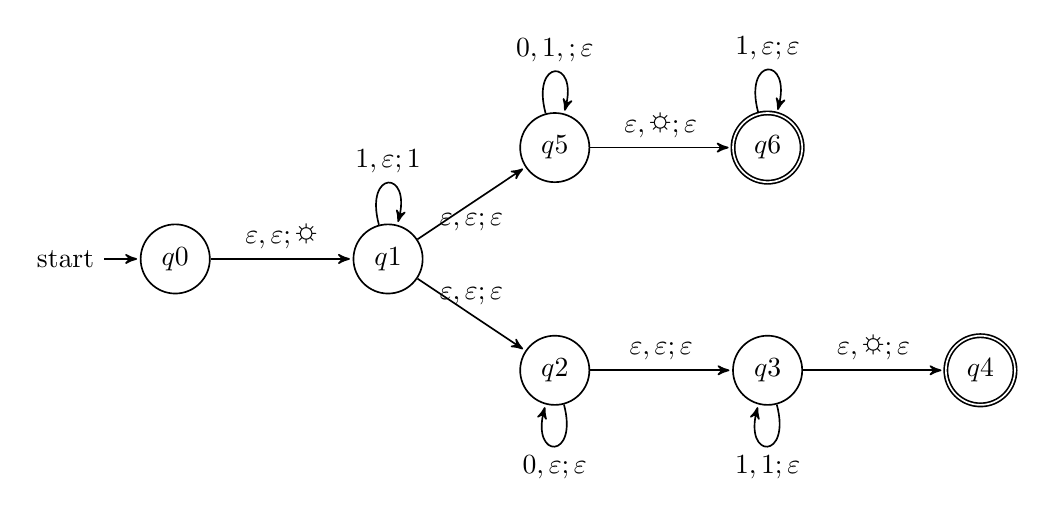
\begin{tikzpicture}[->,>=stealth',shorten >=1pt, auto, node distance=2cm, semithick]
    \tikzstyle{every state}=[text=black, fill=none]
    
    \node[initial,state] (q0)          {$q0$};
    \node[state]         (q1) [right of=q0, xshift=20pt] {$q1$};
    \node[state]         (q2) [below right of=q1, xshift=20pt] {$q2$};
    \node[state]         (q3) [right of=q2, xshift=20pt] {$q3$};
    \node[state,accepting]  (q4) [right of=q3, xshift=20pt] {$q4$};
    \node[state]         (q5) [above right of=q1, xshift=20pt] {$q5$};
    \node[state,accepting]  (q6) [right of=q5, xshift=20pt] {$q6$};
    
    \path (q0) edge [bend left=0] node {$\varepsilon, \varepsilon; \sun$} (q1)
        (q1) edge  [loop above] node {$1, \varepsilon; 1$} (q1)
        (q1) edge [bend left=0] node [below] {$\varepsilon, \varepsilon; \varepsilon$} (q5)
        (q1) edge [bend left=0] node [above]{$\varepsilon, \varepsilon; \varepsilon$} (q2)
        (q5) edge [loop above] node {$0, 1, ; \varepsilon$} (q5)
        (q5) edge [bend left=0] node {$\varepsilon, \sun; \varepsilon$} (q6)
        (q6) edge [loop above] node {$1, \varepsilon; \varepsilon$} (q6)
        (q2) edge [loop below] node {$0, \varepsilon; \varepsilon$} (q2)
        (q2) edge  [bend left=0] node {$\varepsilon, \varepsilon; \varepsilon$} (q3)
        (q3) edge  [loop below] node {$1, 1; \varepsilon$} (q3)
        (q3) edge  [bend left=0] node {$\varepsilon, \sun; \varepsilon$} (q4)
    ;
\end{tikzpicture}
\\
& \\
& \\
\hline
& \\
& \\
& \\
$\{ 0^i 1^j 0^k \mid i,j,k \geq 0 \}$ & \\
& \\
& \\

\end{tabular}
\end{center}
{\it Note: alternate notation is to replace $;$ with $\to$ on arrow labels.}

\newpage
Corollary: for each language $L$ over $\Sigma$, if there is an NFA $N$ with $L(N)=L$
then there is a PDA $M$ with $L(M) = L$

Proof idea: Declare stack alphabet to be $\Gamma = \Sigma$ and then 
don't use stack at all. 


 \vfill

\begin{comment}
{\it Extra practice}: Consider the state diagram of a PDA with input alphabet 
$\Sigma$ and stack alphabet $\Gamma$.

\begin{center}
\begin{tabular}{|c|c|}
\hline
Label & means \\
\hline
$a, b ; c$ when $a \in \Sigma$, $b\in \Gamma$, $c \in \Gamma$ 
& \hspace{3in} \\
& \\
& \\
& \\
& \\
&\\
\hline
$a, \varepsilon ; c$ when $a \in \Sigma$, $c \in \Gamma$ 
& \hspace{3in} \\
& \\
& \\
& \\
& \\
&\\
\hline
$a, b ; \varepsilon$ when $a \in \Sigma$, $b\in \Gamma$
& \hspace{3in} \\
& \\
& \\
& \\
& \\
&\\
\hline
$a, \varepsilon ; \varepsilon$ when $a \in \Sigma$
& \hspace{3in} \\
& \\
& \\
& \\
& \\
&\\
\hline
\end{tabular}
\end{center}


How does the meaning change if $a$ is replaced by $\varepsilon$?
\end{comment}

{\it Big picture}: PDAs are motivated by wanting to add some memory of unbounded size to NFA. How 
do we accomplish a similar enhancement of regular expressions to get a syntactic model that is 
more expressive?

DFA, NFA, PDA: Machines process one input string at a time; the computation of a machine on its input string 
reads the input from left to right.

Regular expressions: Syntactic descriptions of all strings that match a particular pattern; the language 
described by a regular expression is built up recursively according to the expression's syntax

{\bf Context-free grammars}: Rules to produce one string at a time, adding characters from the middle, beginning, 
or end of the final string as the derivation proceeds.\\

\vfill
 \vfill
\section*{Day13}




Definitions below are on pages 101-102.

\vspace{-20pt}

\begin{center}
    \begin{tabular}{|p{2.4in}cp{3.6in}|}
    \hline 
    {\bf Term} & {\bf Typical symbol} & {\bf Meaning} \\
     & or {\bf Notation} & \\
    \hline
    \hline
    {\bf Context-free grammar} (CFG) & $G$ & $G = (V, \Sigma, R, S)$ \\
    The set of {\bf variables}& $V$ & Finite  set of symbols that represent phases in production pattern\\
    The set of {\bf terminals} & $\Sigma$ & Alphabet of symbols of strings generated  by CFG \\
    & & $V \cap \Sigma = \emptyset$ \\
    The set of {\bf rules}& $R$ & Each rule is  $A \to u$ with $A \in V$ and $u  \in (V  \cup \Sigma)^*$\\
    The {\bf start} variable&  $S$  & Usually  on left-hand-side of first/ topmost rule \\
    & &\\
    {\bf Derivation} & $S \Rightarrow \cdots \Rightarrow w$& 
    Sequence  of substitutions in a  CFG (also written $S \Rightarrow^* w$). At each step, we can apply one rule 
    to one occurrence of a variable in the current string by substituting that occurrence of the variable with the 
    right-hand-side of the rule. The derivation must end when the current string has only terminals (no variables)
    because then there are no instances of variables to apply a rule to.\\
    Language {\bf generated} by the context-free grammar $G$ & $L(G)$ &The set of strings for which there is a derivation in $G$. 
    Symbolically: $\{  w \in \Sigma^* \mid S \Rightarrow^* w \}$ i.e. $$\{  w \in \Sigma^* \mid \text{there is  derivation in $G$ that ends
    in $w$} \}$$\\
    {\bf Context-free language} & & A language that is the language generated by some context-free grammar\\
    \hline
    \end{tabular}
\end{center}

\vfill

  
{\bf Examples of context-free grammars, derivations in those grammars, and the languages generated by those grammars}
  
$G_1 =  (\{S\}, \{0\}, R, S)$ with rules
  \begin{align*}
    &S \to 0S\\
    &S \to 0\\
  \end{align*}
  In  $L(G_1)$ \ldots 
  
\vfill

  Not in $L(G_1)$ \ldots 


\vfill

\newpage
  $G_2 =  (\{S\}, \{0,1\}, R, S)$
  \[
  S \to 0S \mid 1S \mid \varepsilon
  \]
  In  $L(G_2)$ \ldots 
  
  \vfill
  
  Not in $L(G_2)$ \ldots 

  \vfill

  $(\{S, T\}, \{0, 1\}, R, S)$ with  rules
  \begin{align*}
  &S \to T1T1T1T \\
  &T \to  0T \mid 1T \mid \varepsilon
  \end{align*}

  In  $L(G_3)$ \ldots 
  
  \vfill
  
  Not in $L(G_3)$ \ldots 

  \vfill

  $G_4 =  (\{A, B\}, \{0, 1\}, R, A)$ with rules
  \[
    A \to 0A0 \mid  0A1 \mid 1A0  \mid 1A1 \mid  1
  \]
  In  $L(G_4)$ \ldots 
  
  \vfill
  
  Not in $L(G_4)$ \ldots 

  \vfill

  
  \newpage
  Design a CFG to generate the  language $\{a^n b^n \mid  n  \geq  0\}$
  
  
  \vfill 


  Design a CFG to generate the  language $\{a^i b^j \mid j \geq i  \geq 0\}$
  
  \vfill
  
  Design a PDA to recognize the  language $\{a^i b^j \mid j \geq i  \geq 0\}$
  
  
  \vfill
  \newpage \vfill
\section*{Day14}



{\bf Theorem  2.20}: A language is  generated by some context-free  grammar
if  and only if it is recognized by some push-down automaton.

Definition: a language is called {\bf context-free} if it is the language generated by a context-free grammar.
The class of all context-free language over a given alphabet $\Sigma$ is called {\bf CFL}.

Consequences:
\begin{itemize}
    \item Quick proof that every regular language is context free 
    \item To prove closure of the class of context-free languages under a given operation, we can choose 
    either of two modes 
    of proof (via CFGs or PDAs) depending on which is easier
    \item To fully specify a PDA we could give its $6$-tuple formal definition or we could give its input 
alphabet, stack alphabet, and state diagram.
An informal description of a PDA is a step-by-step description of how its computations 
would process input strings; the reader should be able to reconstruct the state diagram or formal 
definition precisely from such a descripton. The informal description of a PDA can refer to some 
common modules or subroutines that are computable by PDAs:
\begin{itemize}
  \item PDAs can ``test for emptiness of stack'' without providing details. 
  {\it How?} We can always push a special end-of-stack symbol, $\$$, at the start, before processing
  any input, and then use this symbol as a flag.
  \item PDAs can ``test for end of input'' without providing details.
  {\it How?} We can transform a PDA to one where accepting states are only those reachable 
  when there are no more input symbols.
\end{itemize}

\end{itemize}




\vfill

\newpage
Suppose $L_1$ and $L_2$ are context-free languages over $\Sigma$.  {\bf Goal}:  $L_1 \cup L_2$  is  also context-free.

{\it Approach 1: with  PDAs}

Let $M_1 = ( Q_1, \Sigma, \Gamma_1, \delta_1, q_1, F_1)$ and
$M_2 = ( Q_2, \Sigma, \Gamma_2, \delta_2, q_2, F_2)$ be PDAs with 
$L(M_1) =  L_1$  and  $L(M_2) = L_2$.

Define $M = $

\vfill

{\it Approach  2: with CFGs}

Let $G_1 = (V_1, \Sigma, R_1, S_1)$  and   $G_2 = (V_2, \Sigma, R_2, S_2)$  be CFGs  with
$L(G_1) =  L_1$  and  $L(G_2) = L_2$.

Define $G = $

\vfill

\newpage
Suppose $L_1$ and $L_2$ are context-free languages over $\Sigma$.  {\bf Goal}:  $L_1 \circ L_2$  is  also context-free.


{\it Approach 1: with  PDAs}

Let $M_1 = ( Q_1, \Sigma, \Gamma_1, \delta_1, q_1, F_1)$ and
$M_2 = ( Q_2, \Sigma, \Gamma_2, \delta_2, q_2, F_2)$ be PDAs with 
$L(M_1) =  L_1$  and  $L(M_2) = L_2$.

Define $M = $

\vfill

{\it Approach  2: with CFGs}

Let $G_1 = (V_1, \Sigma, R_1, S_1)$  and   $G_2 = (V_2, \Sigma, R_2, S_2)$  be CFGs  with
$L(G_1) =  L_1$  and  $L(G_2) = L_2$.

Define $G = $

\vfill

{\it Summary}

Over a fixed alphabet $\Sigma$, a language $L$ is {\bf regular}

\vspace{-20pt}
\begin{center}
    iff it is described by some regular expression \\
    iff it is recognized by some DFA\\
    iff it is recognized by some NFA
\end{center}

Over a fixed alphabet $\Sigma$, a language $L$ is {\bf context-free}

\vspace{-20pt}
\begin{center}
    iff it is generated by some CFG\\
    iff it is recognized by some PDA
\end{center}

\vfill

{\bf Fact}: Every regular language is a context-free language.

\vfill

{\bf Fact}: There are context-free languages that are nonregular.

\vfill

{\bf Fact}: There are countably many regular languages.

\vfill

{\bf Fact}: There are countably infinitely many context-free languages.

\vfill

{\it Consequence}: Most languages are {\bf not} context-free!

\vfill

\newpage
{\bf Examples  of non-context-free languages}

\begin{align*}
    &\{ a^n b^n c^n \mid 0 \leq n , n \in \mathbb{Z}\}\\
    &\{ a^i b^j c^k \mid 0 \leq i \leq j \leq k , i \in \mathbb{Z}, j \in \mathbb{Z}, k \in \mathbb{Z}\}\\
    &\{ ww \mid w \in \{0,1\}^* \}
\end{align*}
(Sipser Ex 2.36, Ex 2.37, 2.38)

There is a Pumping Lemma for CFL that can be used to prove a specific language is non-context-free: 
If $A$ is a context-free language, there
is a number $p$ where, if $s$ is any string in $A$ of length at least $p$, then $s$ may be divided 
into five pieces $s = uvxyz$ where (1) for each $i \geq 0$, $uv^ixy^iz \in A$, (2) $|uv|>0$, (3) $|vxy| \leq p$.
{\it We will not go into the details of the proof or application of Pumping Lemma for CFLs this quarter.}


Recall: A set $X$ is said to be {\bf closed} under an operation $OP$ if, for any elements in $X$, applying 
$OP$ to them gives an element in $X$.  


\begin{center}
\begin{tabular}{|c|l|}
\hline
True/False & Closure claim \\
\hline
True &  The set of integers is closed under multiplication. \\
& $\forall x \forall y \left( ~(x \in \mathbb{Z} \wedge y \in \mathbb{Z})\to xy \in \mathbb{Z}~\right)$ \\
\hline
True & For each set $A$, the power set of $A$ is closed under intersection. \\
& $\forall A_1 \forall A_2 \left( ~(A_1 \in \mathcal{P}(A) \wedge A_2 \in \mathcal{P}(A) \in \mathbb{Z}) \to A_1 \cap A_2 \in \mathcal{P}(A)~\right)$ \\
\hline
  & The class of regular languages over $\Sigma$ is closed under complementation. \\
  & \\
 \hline
  & The class of regular languages over $\Sigma$ is closed under union. \\
  & \\
 \hline
  & The class of regular languages over $\Sigma$ is closed under intersection. \\
  & \\
  \hline
  & The class of regular languages over $\Sigma$ is closed under concatenation. \\
  & \\
 \hline
  & The class of regular languages over $\Sigma$ is closed under Kleene star. \\
  & \\
\hline
    & The class of context-free languages over $\Sigma$ is closed under complementation. \\
  & \\
\hline
    & The class of context-free languages over $\Sigma$ is closed under union. \\
  & \\
\hline
    & The class of context-free languages over $\Sigma$ is closed under intersection. \\
  & \\
\hline
    & The class of context-free languages over $\Sigma$ is closed under concatenation. \\
  & \\
\hline
    & The class of context-free languages over $\Sigma$ is closed under Kleene star. \\
  & \\
\hline
\end{tabular}
\end{center}
 \vfill
\section*{Day9}


{\bf Definition and Theorem}: For an alphabet $\Sigma$, a language $L$ over $\Sigma$ is called {\bf regular}
exactly when $L$ is recognized by some DFA, which happens exactly when $L$ is recognized by some NFA, 
and happens exactly when $L$ is described by some regular expression

{\bf We saw that}: The class of regular languages is closed under complementation, union, 
intersection, set-wise concatenation, and Kleene star.

{\it Extra practice}: 

{\bf Disprove}: There is some alphabet $\Sigma$ for which there is 
some language recognized by an NFA but not by any DFA.

\vfill

{\bf Disprove}: There is some alphabet $\Sigma$ for which there is 
some finite language not described by any regular expression over $\Sigma$.

\vfill

{\bf Disprove}: If a language is recognized by an NFA 
then the complement of this language is not recognized by any DFA.

\vfill


{\bf Fix alphabet $\Sigma$. Is every language $L$ over $\Sigma$ regular?}

\begin{center}
\begin{tabular}{c|c}
Set & Cardinality \\
\hline
& \\
$\{0,1\}$ & \\
& \\
$\{0,1\}^*$ & \\
& \\
$\mathcal{P}( \{0,1\})$ & \\
& \\
The set of all languages over $\{0,1\}$ & \\
& \\
The set of all regular expressions over $\{0,1\}$ & \\
& \\
The set of all regular languages over $\{0,1\}$ & \\
& \\
\end{tabular}
\end{center}

\newpage

Strategy: Find an {\bf invariant} property that is true of all regular languages. When analyzing 
a given language, if the invariant is not true about it, then the language is not regular.

\vfill

{\bf Pumping Lemma} (Sipser Theorem 1.70): If $A$ is a regular language, then there
is a number $p$ (a {\it pumping length}) where, if $s$ is any string in $A$ of length at least $p$, 
then $s$ may be divided into three pieces, $s = xyz$ such that
\vspace{-10pt}
\begin{itemize}
\item $|y| > 0$
\item for each $i \geq 0$, $xy^i z \in A$
\item $|xy| \leq p$.
\end{itemize}
\vfill

{\bf Proof idea}: In DFA, the only memory available is in the states. 
Automata can only
``remember'' finitely far in the past and finitely much information, because
they can have only finitely many states. If a computation path of a DFA visits 
the same state more than once, the machine can't tell the difference between 
the first time and future times it visits this state. Thus, if 
a DFA accepts one long string, then it must accept (infinitely) many 
similar strings.
\vfill

{\bf Proof illustration}


\vfill
\vfill


\newpage

{\bf True or False}: A pumping length for $A = \{ 0,1 \}^*$ is $p = 5$.

\vfill


{\bf True or False}: A pumping length for $A = \{ 0,1 \}^*$ is $p = 2$.

\vfill



{\bf True or False}: A pumping length for $A = \{ 0,1 \}^*$ is $p = 105$.

\vfill



Restating {\bf Pumping Lemma}: If $L$ is a regular language, then it  has
a pumping length.


{\bf Contrapositive}: If $L$ has no pumping length, then  it is nonregular.

\vfill

{\Large The Pumping Lemma {\it cannot} be used to prove that a language {\it is} regular.} 

{\Large The Pumping Lemma {\bf can} be used to prove that a language {\it is not} regular.}

{\it Extra practice}: Exercise 1.49 in the book.


\vfill

{\bf Proof strategy}: To prove that a language $L$ is {\bf not} regular, 
\begin{itemize}
    \item Consider an arbitrary positive integer $p$
    \item Prove that $p$ is not a pumping length for $L$
    \item Conclude that $L$ does not have {\it any} pumping length, and therefore it is not regular.
\end{itemize}


{\bf Negation}: A positive integer  $p$  is {\bf not a pumping length} of a language  $L$ over  $\Sigma$  iff
\[
\exists s \left(~  |s| \geq  p \wedge s \in L \wedge \forall x \forall y \forall z  \left( ~\left( s = xyz \wedge 
|y| > 0 \wedge |xy| \leq p~ \right) \to \exists i  (  i \geq 0  \wedge xy^iz  \notin L ) \right) ~\right) 
\] \vfill
\section*{Day10}



{\bf Proof strategy}: To prove that a language $L$ is {\bf not} regular, 
\begin{itemize}
    \item Consider an arbitrary positive integer $p$
    \item Prove that $p$ is not a pumping length for $L$. A positive integer  $p$  is {\bf not a pumping length} of a language  $L$ over  $\Sigma$  iff
    \[
    \exists s \left(~  |s| \geq  p \wedge s \in L \wedge \forall x \forall y \forall z  \left( ~\left( s = xyz \wedge 
    |y| > 0 \wedge |xy| \leq p~ \right) \to \exists i  (  i \geq 0  \wedge xy^iz  \notin L ) \right) ~\right) 
    \]
    {\it Informally: }
    
\vfill

    \item Conclude that $L$ does not have {\it any} pumping length, and therefore it is not regular.
\end{itemize}

\vfill
{\bf Example}: $\Sigma  =  \{0,1\}$, $L = \{ 0^n 1^n \mid n  \geq 0\}$.

Fix $p$ an arbitrary positive integer. List strings that are in $L$ and have length  greater than or equal  to $p$:

\vspace{20pt}

Pick $s = $


Suppose $s = xyz$ with  $|xy|  \leq  p$ and $|y| > 0$.
\begin{center}
\begin{tabular}{|c|}
\hline
 \\
\hspace{4in} \\
\hline
\end{tabular}
\end{center}

Then when $i = \hspace{1in}$, $xy^i z  = \hspace{1in}$

\vfill

\newpage

{\bf Example}: $\Sigma  =  \{0,1\}$, $L = \{w w^{\mathcal{R}} \mid w \in \{0,1\}^*\}$.
Remember that the reverse of a string $w$ is denoted $w^\mathcal{R}$  
and means to write $w$  in  the opposite order, if $w = w_1 \cdots  w_n$ then $w^\mathcal{R} = w_n \cdots  w_1$. Note: $\varepsilon^\mathcal{R} = \varepsilon$.


Fix $p$ an arbitrary positive integer. List strings that are in $L$ and have length  greater than or equal  to $p$:

\vspace{10pt}

Pick $s = $

Suppose $s = xyz$ with  $|xy|  \leq  p$ and $|y| > 0$.
\begin{center}
\begin{tabular}{|c|}
\hline
 \\
\hspace{4in} \\
\hline
\end{tabular}
\end{center}
Then when $i = \hspace{1in}$, $xy^i z  = \hspace{1in}$


\vfill


{\bf Example}: $\Sigma  =  \{0,1\}$, $L = \{0^j1^k  \mid j \geq k  \geq 0\}$.

Fix $p$ an arbitrary positive integer. List strings that are in $L$ and have length  greater than or equal  to $p$:

\vspace{10pt}

Pick $s = $


Suppose $s = xyz$ with  $|xy|  \leq  p$ and $|y| > 0$.
\begin{center}
\begin{tabular}{|c|}
\hline
 \\
\hspace{4in} \\
\hline
\end{tabular}
\end{center}
Then when $i = \hspace{1in}$, $xy^i z  = \hspace{1in}$


\vfill


{\bf Example}: $\Sigma  =  \{0,1\}$, $L = \{0^n1^m0^n  \mid m,n  \geq 0\}$.

Fix $p$ an arbitrary positive integer. List strings that are in $L$ and have length  greater than or equal  to $p$:

\vspace{10pt}

Pick $s = $


Suppose $s = xyz$ with  $|xy|  \leq  p$ and $|y| > 0$.
\begin{center}
\begin{tabular}{|c|}
\hline
 \\
\hspace{4in} \\
\hline
\end{tabular}
\end{center}
Then when $i = \hspace{1in}$, $xy^i z  = \hspace{1in}$

\newpage
{\it Extra practice}:


\begin{center}
    \begin{tabular}{c|c| c| c}
    Language & $s \in L$ & $s \notin L$ & Is the language regular or nonregular?  \\
    \hline
     & \hspace{1in} & \hspace{1in}  &  \\
    $\{a^nb^n \mid 0  \leq n  \leq 5 \}$ & & & \\
     & & & \\
    $\{b^n a^n \mid  n  \geq 2\}$  & & & \\
     & & & \\
    $\{a^m b^n \mid  0 \leq m\leq n\}$  & & & \\
     & & & \\
    $\{a^m b^n \mid  m \geq n+3,  n \geq 0\}$  & & & \\
     & & & \\
    $\{b^m a^n \mid  m \geq 1, n \geq  3\}$  & & & \\
     & & & \\
    $\{ w  \in \{a,b\}^* \mid w = w^\mathcal{R} \}$ & & & \\
     & & & \\ 
    $\{ ww^\mathcal{R} \mid w\in \{a,b\}^* \}$ & & & \\
     & & & \\ 
    \end{tabular}
\end{center}
     \vfill
\section*{Day11}


Regular sets are not the end of the story
\begin{itemize}
    \item Many nice / simple / important sets are not regular
    \item Limitation of the finite-state automaton model: Can't ``count", Can only remember finitely far into the past,
    Can't backtrack, Must make decisions in ``real-time"
    \item We know actual computers are more powerful than this model...
\end{itemize}

The {\bf next} model of computation. Idea: allow some memory of unbounded size. How? 
\begin{itemize}
    \item To generalize regular expressions: {\bf context-free grammars}\\
    \item To generalize NFA: {\bf Pushdown automata}, which is like an NFA with access to a stack: 
    Number of states is fixed, number of entries in stack is unbounded. At each step
    (1) Transition to new state based on current state, letter read, and top letter of stack, then
    (2) (Possibly) push or pop a letter to (or from) top of stack. Accept a string iff
    there is some sequence of states and some sequence of stack contents 
    which helps the PDA processes the entire input string and ends in an accepting state.
\end{itemize}

\vfill

\vfill

Is there a PDA that recognizes the nonregular language $\{0^n1^n \mid n \geq 0 \}$?

\vfill

\newpage

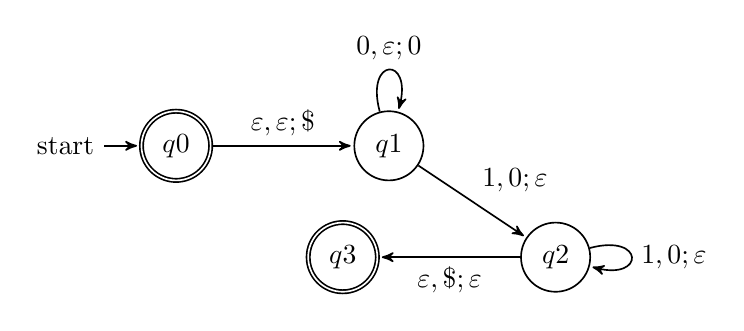
\begin{tikzpicture}[->,>=stealth',shorten >=1pt, auto, node distance=2cm, semithick]
    \tikzstyle{every state}=[text=black, fill=none]
    
    \node[initial,state,accepting] (q0)          {$q0$};
    \node[state]         (q1) [right of=q0, xshift=20pt] {$q1$};
    \node[state]         (q2) [below right of=q1, xshift=20pt] {$q2$};
    \node[state,accepting]         (q3) [left of=q2, xshift=-20pt] {$q3$};
    
    \path (q0) edge [bend left=0] node {$\varepsilon, \varepsilon; \$$} (q1)
        (q1) edge  [loop above] node {$0, \varepsilon; 0$} (q1)
        (q1) edge [bend left=0] node {$1, 0; \varepsilon$} (q2)
        (q2) edge  [loop right] node {$1, 0; \varepsilon$} (q2)
        (q2) edge  [bend left=0] node {$\varepsilon, \$; \varepsilon$} (q3)
    ;
\end{tikzpicture}

The PDA with state diagram above can be informally described as:
\begin{quote}
    Read symbols from the input. As each 0 is read, push it onto the stack. 
    As soon as 1s are seen, pop a 0 off the stack for each 1 read. 
    If the stack becomes empty and we are at the end of the input string, accept the input. 
    If the stack becomes empty and there are 1s left to read, 
    or if 1s are finished while the stack still contains 0s, or if any 0s
    appear in the string following 1s, 
    reject the input.
\end{quote}
    

Trace a computation of this PDA on the input string $01$.

\vfill
    
{\it Extra practice}: Trace the computations of this PDA on the input string $011$.

\vfill

\newpage
A PDA recognizing the set $\{ \hspace{1.5 in} \}$ can be informally described as:
\begin{quote}
    Read symbols from the input. As each 0 is read, push it onto the stack. 
    As soon as 1s are seen, pop a 0 off the stack for each 1 read. 
    If the stack becomes empty and there is exactly one 1 left to read, read that 1 and accept the input. 
    If the stack becomes empty and there are either zero or more than one 1s left to read, 
    or if the 1s are finished while the stack still contains 0s, or if any 0s appear in the input following 1s, 
    reject the input.
\end{quote}
Modify the state diagram below to get a PDA that implements this description:

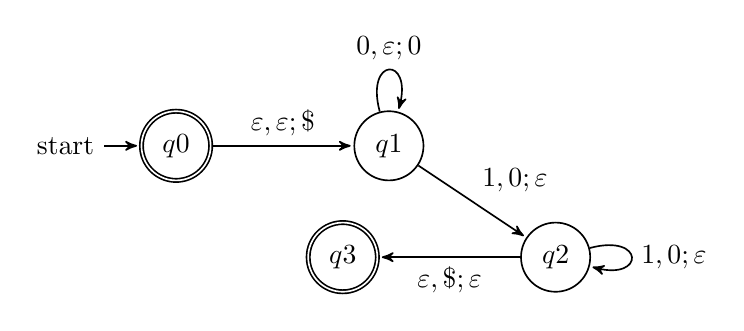
\begin{tikzpicture}[->,>=stealth',shorten >=1pt, auto, node distance=2cm, semithick]
    \tikzstyle{every state}=[text=black, fill=none]
    
    \node[initial,state,accepting] (q0)          {$q0$};
    \node[state]         (q1) [right of=q0, xshift=20pt] {$q1$};
    \node[state]         (q2) [below right of=q1, xshift=20pt] {$q2$};
    \node[state,accepting]         (q3) [left of=q2, xshift=-20pt] {$q3$};
    
    \path (q0) edge [bend left=0] node {$\varepsilon, \varepsilon; \$$} (q1)
        (q1) edge  [loop above] node {$0, \varepsilon; 0$} (q1)
        (q1) edge [bend left=0] node {$1, 0; \varepsilon$} (q2)
        (q2) edge  [loop right] node {$1, 0; \varepsilon$} (q2)
        (q2) edge  [bend left=0] node {$\varepsilon, \$; \varepsilon$} (q3)
    ;
\end{tikzpicture}
    
 \vfill
\section*{Day15}


We are ready to introduce a formal model that will capture a notion of general purpose computation.
\begin{itemize}
\item {\it Similar to DFA, NFA, PDA}: input will be an arbitrary string over a fixed alphabet.
\item {\it Different from NFA, PDA}: machine is deterministic.
\item {\it Different from DFA, NFA, PDA}: read-write head can move both to the left and to the right,
and can extend to the right past the original input.
\item {\it Similar to DFA, NFA, PDA}: transition function drives computation one step at a time 
by moving within a finite set of states, always starting at designated start state.
\item {\it Different from DFA, NFA, PDA}: the special states for rejecting and accepting take effect immediately.
\end{itemize}

\vspace{-10pt}

(See more details: Sipser p. 166)

\vfill

Formally: a  Turing machine is $M= (Q, \Sigma, \Gamma, \delta, q_0, q_{accept}, q_{reject})$ 
where $\delta$ is the {\bf transition function} 
\[
  \delta: Q\times \Gamma \to Q \times \Gamma \times \{L, R\}
\]
The {\bf computation} of $M$ on a string $w$ over $\Sigma$  is:

\vspace{-10pt}

\begin{itemize}
\setlength{\itemsep}{0pt}
\item Read/write head starts at leftmost position on tape. 
\item Input string is written on $|w|$-many leftmost cells of tape, 
rest of  the tape cells have  the blank symbol. {\bf Tape alphabet} 
is $\Gamma$ with $\textvisiblespace\in \Gamma$ and $\Sigma \subseteq \Gamma$.
The blank symbol $\textvisiblespace \notin \Sigma$.
\item Given current state of machine and current symbol being read at the tape head, 
the machine transitions to next state, writes a symbol to the current position  of the 
tape  head (overwriting existing symbol), and moves the tape head L or R (if possible). 
\item Computation ends {\bf if and when} machine enters either the accept or the reject state.
This is called {\bf halting}.
Note: $q_{accept} \neq q_{reject}$.
\end{itemize}

The {\bf language recognized by the  Turing machine} $M$,  is  $L(M) = \{ w \in \Sigma^* \mid w \textrm{ is accepted by } M\}$,
which is defined as
\[
  \{ w \in \Sigma^* \mid \textrm{computation of $M$ on $w$ halts after entering the accept state}\}
\]




\newpage
\begin{multicols}{2}
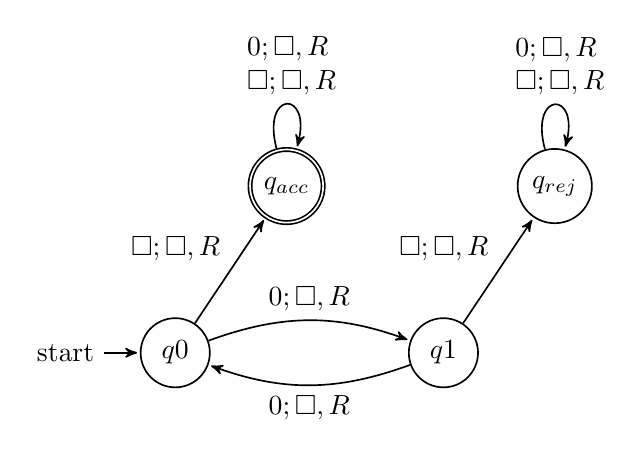
\begin{tikzpicture}[->,>=stealth',shorten >=1pt, auto, node distance=2cm, semithick]
  \tikzstyle{every state}=[text=black, fill=none]
  
  \node[initial,state] (q0)          {$q0$};
  \node[state]         (q1) [right of=q0, xshift=40pt] {$q1$};
  \node[state,accepting]         (qacc) [above right of=q0, yshift=20pt] {$q_{acc}$};
  \node[state]         (qrej) [above right of=q1,yshift=20pt] {$q_{rej}$};
  
  \path (q0) edge [bend left=0] node {$\square; \square, R$} (qacc)
      (q0) edge  [bend left=20] node {$0; \square, R$} (q1)
      (q1) edge [bend left=20] node {$0; \square, R$} (q0)
      (q1) edge [bend left=0] node {$\square; \square, R$} (qrej)
      (qacc) edge  [loop above] node {\parbox{1cm}{$0; \square, R$\newline $\square; \square, R$}} (qacc)
      (qrej) edge  [loop above] node {\parbox{1cm}{$0; \square, R$\newline $\square; \square, R$}}  (qrej)
  ;
\end{tikzpicture}
\columnbreak

Formal definition:

\vspace{10pt}

Sample computation: 

\begin{tabular}{|c|c|c|c|c|c|c|}
\hline
\multicolumn{1}{|c}{$q0\downarrow$} &  \multicolumn{6}{c|}{\phantom{A}}\\
\hline
$0$ & $0$  & $0$ & $\textvisiblespace $& $\textvisiblespace $& $\textvisiblespace $&  $\textvisiblespace $\\
\hline
\multicolumn{7}{|c|}{\phantom{A}}\\
\hline
\phantom{AA} & \phantom{AA}& \phantom{AA}& \phantom{AA}& \phantom{AA}& \phantom{AA}& \phantom{AA} \\
\hline
\multicolumn{7}{|c|}{\phantom{A}}\\
\hline
\phantom{AA} & \phantom{AA}& \phantom{AA}& \phantom{AA}& \phantom{AA}& \phantom{AA}& \phantom{AA} \\
\hline
\multicolumn{7}{|c|}{\phantom{A}}\\
\hline
\phantom{AA} & \phantom{AA}& \phantom{AA}& \phantom{AA}& \phantom{AA}& \phantom{AA}& \phantom{AA} \\
\hline
\multicolumn{7}{|c|}{\phantom{A}}\\
\hline
\phantom{AA} & \phantom{AA}& \phantom{AA}& \phantom{AA}& \phantom{AA}& \phantom{AA}& \phantom{AA} \\
\hline
\end{tabular}
\end{multicols}
\vfill

The language recognized by this machine is \ldots

\vfill
 

{\bf Describing  Turing machines} (Sipser p. 185) To define a Turing machine, we could give a 
\begin{itemize}
\item {\bf Formal definition}: the $7$-tuple of parameters including set of states, 
input alphabet, tape alphabet, transition function, start state, accept state, and reject state; or,
\item {\bf Implementation-level definition}: English prose that describes the Turing machine head 
movements relative to contents of tape, and conditions for accepting / rejecting based on those contents.
\item {\bf High-level description}: description of algorithm (precise sequence of instructions), 
without implementation details of machine. As part of this description, can ``call" and run 
another TM as a subroutine.
\end{itemize}
  
\newpage
Fix $\Sigma = \{0,1\}$, $\Gamma = \{ 0, 1, \textvisiblespace\}$ for the Turing machines with  the following state diagrams:
  
\begin{center}
  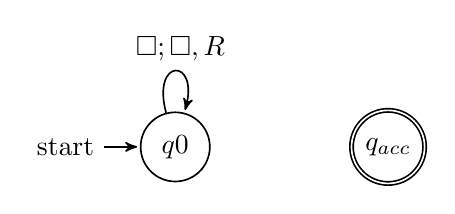
\begin{tikzpicture}[->,>=stealth',shorten >=1pt, auto, node distance=2cm, semithick]
    \tikzstyle{every state}=[text=black, fill=none]
    
    \node[initial,state] (q0)          {$q0$};
    \node[state,accepting]         (qacc) [right of=q0, xshift=20pt] {$q_{acc}$};
    
    \path (q0) edge  [loop above] node {\parbox{1cm}{$\square; \square, R$}} (q0)
    ;
  \end{tikzpicture}
\end{center}

Example of string accepted: \\
Example of string rejected: \\


Implementation-level description

\vfill

High-level description

\vfill

\begin{center}
  \begin{tikzpicture}[->,>=stealth',shorten >=1pt, auto, node distance=2cm, semithick]
    \tikzstyle{every state}=[text=black, fill=none]
    
    \node[initial,state] (qrej)          {$q_{rej}$};
    \node[state,accepting]         (qacc) [right of=q0, xshift=20pt] {$q_{acc}$};
  \end{tikzpicture}
\end{center}

Example of string accepted: \\
Example of string rejected: \\


Implementation-level description

\vfill

High-level description

\vfill

\newpage
\begin{center}
  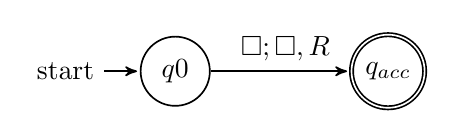
\begin{tikzpicture}[->,>=stealth',shorten >=1pt, auto, node distance=2cm, semithick]
    \tikzstyle{every state}=[text=black, fill=none]
    
    \node[initial,state] (q0)          {$q0$};
    \node[state,accepting]         (qacc) [right of=q0, xshift=20pt] {$q_{acc}$};
    
    \path (q0) edge  [bend left=0] node {\parbox{1cm}{$\square; \square, R$}} (qacc)
    ;
  \end{tikzpicture}
\end{center}

Example of string accepted: \\
Example of string rejected: \\


Implementation-level description

\vfill

High-level description

\vfill

\begin{center}
  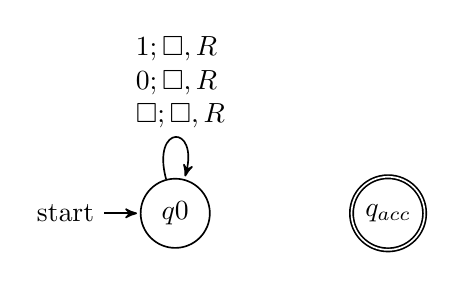
\begin{tikzpicture}[->,>=stealth',shorten >=1pt, auto, node distance=2cm, semithick]
    \tikzstyle{every state}=[text=black, fill=none]
    
    \node[initial,state] (q0)          {$q0$};
    \node[state,accepting]         (qacc) [right of=q0, xshift=20pt] {$q_{acc}$};
    
    \path (q0) edge  [loop above] node {\parbox{1cm}{$1; \square, R$\\$0; \square, R$\\$\square; \square, R$}} (q0)
    ;
  \end{tikzpicture}
\end{center}

Example of string accepted: \\
Example of string rejected: \\


Implementation-level description

\vfill

High-level description

\vfill

\newpage
 \vfill
\section*{Day16}



{\it Sipser Figure  3.10}

{\bf Conventions in state diagram of TM}: $b \to R$ label means $b \to b, R$ and
all arrows missing from diagram represent transitions with output $(q_{reject}, \textvisiblespace , R)$

\begin{multicols}{2}
\vspace{-20pt}
\begin{center}
\includegraphics[width=4in]{Lect13TM3.png}
\end{center}

Implementation level description of this machine:
\begin{quote}
Zig-zag across tape to corresponding positions on either side of $\#$ to check whether the 
characters in these positions agree. If they do not, or if there is no $\#$, reject. If they 
do, cross them off.

Once all symbols to the left of the $\#$ are crossed off, check for any un-crossed-off symbols 
to the right of $\#$; if there are any, reject; if there aren't, accept.
\end{quote}

The language recognized by this machine is
\[
  \{ w \# w \mid w \in \{0,1\}^* \}
\]

\columnbreak

Computation on  input  string  $01\#01$

\begin{tabular}{|c|c|c|c|c|c|c|}
\hline
\multicolumn{1}{|c}{$q_1 \downarrow$} &  \multicolumn{6}{c|}{\phantom{A}}\\
\hline
$0$ & $1$  & $\#$  & $0$ & $1$ & $\textvisiblespace $& $\textvisiblespace $\\
\hline
  \multicolumn{7}{|c|}{\phantom{A}}\\
  \hline
  \phantom{AA} & \phantom{AA}& \phantom{AA}& \phantom{AA}& \phantom{AA}& \phantom{AA}& \phantom{AA} \\
  \hline
  \multicolumn{7}{|c|}{\phantom{A}}\\
  \hline
  \phantom{AA} & \phantom{AA}& \phantom{AA}& \phantom{AA}& \phantom{AA}& \phantom{AA}& \phantom{AA} \\
  \hline
  \multicolumn{7}{|c|}{\phantom{A}}\\
  \hline
  \phantom{AA} & \phantom{AA}& \phantom{AA}& \phantom{AA}& \phantom{AA}& \phantom{AA}& \phantom{AA} \\
  \hline
  \multicolumn{7}{|c|}{\phantom{A}}\\
  \hline
  \phantom{AA} & \phantom{AA}& \phantom{AA}& \phantom{AA}& \phantom{AA}& \phantom{AA}& \phantom{AA} \\
  \hline
  \multicolumn{7}{|c|}{\phantom{A}}\\
  \hline
  \phantom{AA} & \phantom{AA}& \phantom{AA}& \phantom{AA}& \phantom{AA}& \phantom{AA}& \phantom{AA} \\
  \hline
  \multicolumn{7}{|c|}{\phantom{A}}\\
  \hline
  \phantom{AA} & \phantom{AA}& \phantom{AA}& \phantom{AA}& \phantom{AA}& \phantom{AA}& \phantom{AA} \\
  \hline
  \multicolumn{7}{|c|}{\phantom{A}}\\
  \hline
  \phantom{AA} & \phantom{AA}& \phantom{AA}& \phantom{AA}& \phantom{AA}& \phantom{AA}& \phantom{AA} \\
  \hline
  \multicolumn{7}{|c|}{\phantom{A}}\\
  \hline
  \phantom{AA} & \phantom{AA}& \phantom{AA}& \phantom{AA}& \phantom{AA}& \phantom{AA}& \phantom{AA} \\
  \hline
  \multicolumn{7}{|c|}{\phantom{A}}\\
  \hline
  \phantom{AA} & \phantom{AA}& \phantom{AA}& \phantom{AA}& \phantom{AA}& \phantom{AA}& \phantom{AA} \\
  \hline
  \multicolumn{7}{|c|}{\phantom{A}}\\
  \hline
  \phantom{AA} & \phantom{AA}& \phantom{AA}& \phantom{AA}& \phantom{AA}& \phantom{AA}& \phantom{AA} \\
  \hline
  \multicolumn{7}{|c|}{\phantom{A}}\\
  \hline
  \phantom{AA} & \phantom{AA}& \phantom{AA}& \phantom{AA}& \phantom{AA}& \phantom{AA}& \phantom{AA} \\
  \hline
  \multicolumn{7}{|c|}{\phantom{A}}\\
  \hline
  \phantom{AA} & \phantom{AA}& \phantom{AA}& \phantom{AA}& \phantom{AA}& \phantom{AA}& \phantom{AA} \\
  \hline
  \multicolumn{7}{|c|}{\phantom{A}}\\
  \hline
  \phantom{AA} & \phantom{AA}& \phantom{AA}& \phantom{AA}& \phantom{AA}& \phantom{AA}& \phantom{AA} \\
  \hline
  \multicolumn{7}{|c|}{\phantom{A}}\\
  \hline
  \phantom{AA} & \phantom{AA}& \phantom{AA}& \phantom{AA}& \phantom{AA}& \phantom{AA}& \phantom{AA} \\
  \hline
  \multicolumn{7}{|c|}{\phantom{A}}\\
  \hline
  \phantom{AA} & \phantom{AA}& \phantom{AA}& \phantom{AA}& \phantom{AA}& \phantom{AA}& \phantom{AA} \\
  \hline
  \multicolumn{7}{|c|}{\phantom{A}}\\
  \hline
  \phantom{AA} & \phantom{AA}& \phantom{AA}& \phantom{AA}& \phantom{AA}& \phantom{AA}& \phantom{AA} \\
  \hline
  \multicolumn{7}{|c|}{\phantom{A}}\\
  \hline
  \phantom{AA} & \phantom{AA}& \phantom{AA}& \phantom{AA}& \phantom{AA}& \phantom{AA}& \phantom{AA} \\
  \hline
  \multicolumn{7}{|c|}{\phantom{A}}\\
  \hline
  \phantom{AA} & \phantom{AA}& \phantom{AA}& \phantom{AA}& \phantom{AA}& \phantom{AA}& \phantom{AA} \\
  \hline
  \end{tabular}
\end{multicols}

\begin{multicols}{2}
High-level description of this machine is

\vfill


{\it Recall:} 
High-level descriptions of  Turing machine algorithms are written as indented text within quotation marks.   
Stages of the algorithm are typically numbered consecutively.
The first line specifies the input to the machine, which must be a string.

\columnbreak

{\it Extra practice}

Computation on  input  string  $01\#1$

\begin{tabular}{|c|c|c|c|c|c|c|}
\hline
\multicolumn{1}{|c}{$q_1\downarrow$} &  \multicolumn{6}{c|}{\phantom{A}}\\
\hline
$0$ & $1$  & $\#$  & $1$ & $\textvisiblespace $& $\textvisiblespace $&  $\textvisiblespace $\\
\hline
\multicolumn{7}{|c|}{\phantom{A}}\\
\hline
\phantom{AA} & \phantom{AA}& \phantom{AA}& \phantom{AA}& \phantom{AA}& \phantom{AA}& \phantom{AA} \\
\hline
\multicolumn{7}{|c|}{\phantom{A}}\\
\hline
\phantom{AA} & \phantom{AA}& \phantom{AA}& \phantom{AA}& \phantom{AA}& \phantom{AA}& \phantom{AA} \\
\hline
\multicolumn{7}{|c|}{\phantom{A}}\\
\hline
\phantom{AA} & \phantom{AA}& \phantom{AA}& \phantom{AA}& \phantom{AA}& \phantom{AA}& \phantom{AA} \\
\hline
\multicolumn{7}{|c|}{\phantom{A}}\\
\hline
\phantom{AA} & \phantom{AA}& \phantom{AA}& \phantom{AA}& \phantom{AA}& \phantom{AA}& \phantom{AA} \\
\hline
\multicolumn{7}{|c|}{\phantom{A}}\\
\hline
\phantom{AA} & \phantom{AA}& \phantom{AA}& \phantom{AA}& \phantom{AA}& \phantom{AA}& \phantom{AA} \\
\hline
\multicolumn{7}{|c|}{\phantom{A}}\\
\hline
\phantom{AA} & \phantom{AA}& \phantom{AA}& \phantom{AA}& \phantom{AA}& \phantom{AA}& \phantom{AA} \\
\hline
\multicolumn{7}{|c|}{\phantom{A}}\\
\hline
\phantom{AA} & \phantom{AA}& \phantom{AA}& \phantom{AA}& \phantom{AA}& \phantom{AA}& \phantom{AA} \\
\hline
\multicolumn{7}{|c|}{\phantom{A}}\\
\hline
\phantom{AA} & \phantom{AA}& \phantom{AA}& \phantom{AA}& \phantom{AA}& \phantom{AA}& \phantom{AA} \\
\hline
\multicolumn{7}{|c|}{\phantom{A}}\\
\hline
\phantom{AA} & \phantom{AA}& \phantom{AA}& \phantom{AA}& \phantom{AA}& \phantom{AA}& \phantom{AA} \\
\hline
\multicolumn{7}{|c|}{\phantom{A}}\\
\hline
\phantom{AA} & \phantom{AA}& \phantom{AA}& \phantom{AA}& \phantom{AA}& \phantom{AA}& \phantom{AA} \\
\hline
\multicolumn{7}{|c|}{\phantom{A}}\\
\hline
\phantom{AA} & \phantom{AA}& \phantom{AA}& \phantom{AA}& \phantom{AA}& \phantom{AA}& \phantom{AA} \\
\hline
\multicolumn{7}{|c|}{\phantom{A}}\\
\hline
\phantom{AA} & \phantom{AA}& \phantom{AA}& \phantom{AA}& \phantom{AA}& \phantom{AA}& \phantom{AA} \\
\hline
\multicolumn{7}{|c|}{\phantom{A}}\\
\hline
\phantom{AA} & \phantom{AA}& \phantom{AA}& \phantom{AA}& \phantom{AA}& \phantom{AA}& \phantom{AA} \\
\hline
\multicolumn{7}{|c|}{\phantom{A}}\\
\hline
\phantom{AA} & \phantom{AA}& \phantom{AA}& \phantom{AA}& \phantom{AA}& \phantom{AA}& \phantom{AA} \\
\hline
\multicolumn{7}{|c|}{\phantom{A}}\\
\hline
\phantom{AA} & \phantom{AA}& \phantom{AA}& \phantom{AA}& \phantom{AA}& \phantom{AA}& \phantom{AA} \\
\hline
\multicolumn{7}{|c|}{\phantom{A}}\\
\hline
\phantom{AA} & \phantom{AA}& \phantom{AA}& \phantom{AA}& \phantom{AA}& \phantom{AA}& \phantom{AA} \\
\hline
\multicolumn{7}{|c|}{\phantom{A}}\\
\hline
\phantom{AA} & \phantom{AA}& \phantom{AA}& \phantom{AA}& \phantom{AA}& \phantom{AA}& \phantom{AA} \\
\hline
\multicolumn{7}{|c|}{\phantom{A}}\\
\hline
\phantom{AA} & \phantom{AA}& \phantom{AA}& \phantom{AA}& \phantom{AA}& \phantom{AA}& \phantom{AA} \\
\hline
\multicolumn{7}{|c|}{\phantom{A}}\\
\hline
\phantom{AA} & \phantom{AA}& \phantom{AA}& \phantom{AA}& \phantom{AA}& \phantom{AA}& \phantom{AA} \\
\hline
\multicolumn{7}{|c|}{\phantom{A}}\\
\hline
\phantom{AA} & \phantom{AA}& \phantom{AA}& \phantom{AA}& \phantom{AA}& \phantom{AA}& \phantom{AA} \\
\hline
\end{tabular}

\end{multicols}
\newpage



A language $L$ is {\bf recognized by} a Turing machine $M$ means

\vfill

A Turing  machine  $M$ {\bf  recognizes} a language $L$ means

\vfill

A Turing machine $M$ is a {\bf decider}  means

\vfill

A language  $L$ is {\bf decided by} a Turing  machine  $M$  means

\vfill

A  Turing machine $M$ {\bf decides} a language $L$ means

\vfill

Fix $\Sigma = \{0,1\}$, $\Gamma = \{ 0, 1, \textvisiblespace\}$ for the Turing machines with  the following state diagrams:
  
  \begin{center}
  \begin{tabular}{|c|c|}
  \hline
  \hspace{0.8in}
  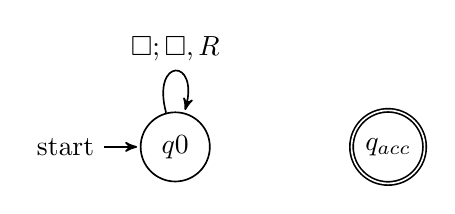
\begin{tikzpicture}[->,>=stealth',shorten >=1pt, auto, node distance=2cm, semithick]
    \tikzstyle{every state}=[text=black, fill=none]
    
    \node[initial,state] (q0)          {$q0$};
    \node[state,accepting]         (qacc) [right of=q0, xshift=20pt] {$q_{acc}$};
    
    \path (q0) edge  [loop above] node {$\square; \square, R$} (qacc)
    ;
  \end{tikzpicture}
\phantom{\hspace{0.8in}}&\hspace{0.8in} 
  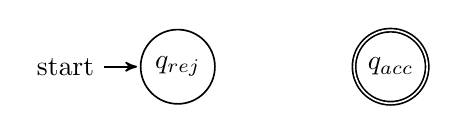
\begin{tikzpicture}[->,>=stealth',shorten >=1pt, auto, node distance=2cm, semithick]
    \tikzstyle{every state}=[text=black, fill=none]
    
    \node[initial,state] (qrej)          {$q_{rej}$};
    \node[state,accepting]         (qacc) [right of=qrej, xshift=20pt] {$q_{acc}$};
  \end{tikzpicture}
  \phantom{\hspace{0.8in}}\\
  Decider? Yes~~~/ ~~~No
  &Decider? Yes~~~/ ~~~No\\
  & \\
  \hline

  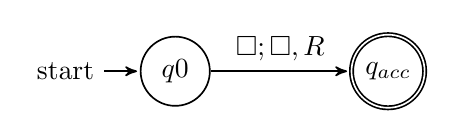
\begin{tikzpicture}[->,>=stealth',shorten >=1pt, auto, node distance=2cm, semithick]
    \tikzstyle{every state}=[text=black, fill=none]
    
    \node[initial,state] (q0)          {$q0$};
    \node[state,accepting]         (qacc) [right of=q0, xshift=20pt] {$q_{acc}$};

    \path (q0) edge [bend left=0] node {$\square; \square, R$} (qacc)
    ;
  \end{tikzpicture} & 
  
  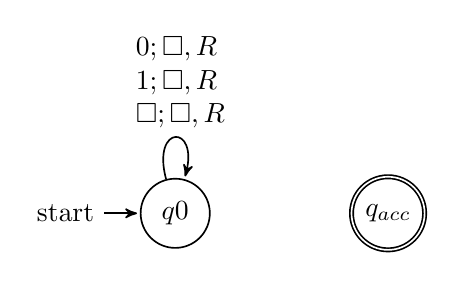
\begin{tikzpicture}[->,>=stealth',shorten >=1pt, auto, node distance=2cm, semithick]
    \tikzstyle{every state}=[text=black, fill=none]
    
    \node[initial,state] (q0)          {$q0$};
    \node[state,accepting]         (qacc) [right of=q0, xshift=20pt] {$q_{acc}$};
    
    \path (q0) edge  [loop above] node {\parbox{1cm}{$0; \square, R$\newline$1; \square, R$\newline $\square; \square, R$}} (q0)
    ;
  \end{tikzpicture}\\
  Decider? Yes~~~/ ~~~No
  &Decider? Yes~~~/ ~~~No\\
  & \\
  
  \hline
  \end{tabular}
  \end{center}
  \newpage

 \vfill
\section*{Day17}




A {\bf Turing-recognizable} language is a set of strings that 
is the language recognized by some Turing machine. We also 
say that such languages are recognizable.

A {\bf Turing-decidable} language is a set of strings that 
is the language recognized by some decider. We also 
say that such languages are decidable.


An {\bf unrecognizable} language is a language that is not Turing-recognizable.

An {\bf undecidable} language is a language that is not Turing-decidable.

\vfill

{\bf  True} or {\bf False}: Any  decidable language  is  also  recognizable.

\vfill

{\bf  True} or {\bf False}: Any  recognizable language  is  also  decidable.

\vfill

{\bf  True} or {\bf False}: Any  undecidable language  is  also  unrecognizable.

\vfill

{\bf  True} or {\bf False}: Any  unrecognizable language  is  also  undecidable.

\vfill

\newpage


{\bf True} or {\bf False}: The class of Turing-decidable languages is closed under complementation.

\vfill

Using formal definition:
\vfill

Using high-level description:
\vfill


{\bf  Church-Turing Thesis} (Sipser p. 183): The informal notion of algorithm is formalized completely  and correctly by the 
formal definition of a  Turing machine. In other words: all reasonably expressive models of 
computation are equally expressive with the standard Turing machine.
 \vfill
\end{document}